\chapter{Normalization and Schema Design}
\hrulefill

\section{Normalization}
\lipsum[1][1-3] 

\subsection{First Normal Form}
\lipsum[1][1] \\ [\baselineskip]
\lipsum[1][2] \\ [\baselineskip]
\lipsum[1][3] \\ [\baselineskip]

\subsection{Second Normal Form}
\lipsum[1][1] \\ [\baselineskip]
\lipsum[1][2] \\ [\baselineskip]
\lipsum[1][3] \\ [\baselineskip]

\subsection{Third Normal Form}
\lipsum[1][1] \\ [\baselineskip]
\lipsum[1][2] \\ [\baselineskip]
\lipsum[1][3] \\ [\baselineskip]

\subsection{Final Table}
\lipsum[1][1] \\ [\baselineskip]
\lipsum[1][2] \\ [\baselineskip]
\lipsum[1][3] \\ [\baselineskip]

\clearpage

\section{Schema Diagram}
\begin{figure}[h]
    \centering
    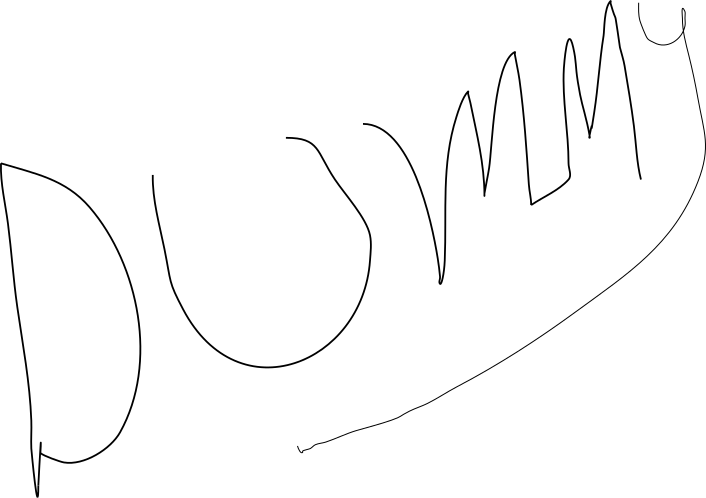
\includegraphics[width=0.9\textwidth]{images/dummy}
    \caption{Schema Diagram}
    \label{fig:Schema Diagram}
\end{figure}